%===============================================================
% Author: Rodolfo Ferro Pérez
% Email: ferro@cimat.mx
% Twitter: @FerroRodolfo
%
% This document was originally created by Rodolfo Ferro, for
% his talk in FLISoL 2017 at Instituto Tecnológico de León.
% Any usage of this document or its contents must be granted by
% the author. You can contact him via email or Twitter.
%===============================================================

\documentclass{beamer}
\usetheme{metropolis} % Use metropolis theme

\usepackage[many]{tcolorbox}
\usepackage{wrapfig}

\title{Primeros pasos con Python:}
\subtitle{Manipulando imágenes}
\author{Rodolfo Ferro\\{\footnotesize \textsc{@FerroRodolfo}}}
\institute{Universidad de Guanajuato\\ CIMAT A.C.\\
\begin{wrapfigure}{r}{0.3\textwidth}
  \vspace{-30pt}
  \begin{center}
    
\includegraphics[width=0.3\textwidth]{imgs/flisol}
  \end{center}
\end{wrapfigure}
}
\date{Abril 29, 2017}
\begin{document}
  % Title slide:
  \maketitle

  % Table of contents:
  \begin{frame}{Tabla de contenido}
    \setbeamertemplate{section in toc}[sections numbered]
    \tableofcontents[hideallsubsections]
  \end{frame}

  % First section: Acerca de Python
  \section{Sobre Python}
  \begin{frame}[standout]
    \textit{"Python es un lenguaje interpretado, sencillo, versátil y poderoso.
    La belleza del lenguaje radica en su sintaxis."}\\
    \vspace{1.4cm}
    
\includegraphics[scale=0.017]{imgs/python}
  \end{frame}

  \begin{frame}{Un poco de historia I}
    \begin{itemize}
      \item Python fue creado a inicios de los 90's por Guido van Rossum en el
      \textit{Stichting Mathematisch Centrum} (CWI), en los Países Bajos, como
      un sucesor del lenguaje ABC.

      \item Guido sigue siendo el principal autor, aunque incluye muchas
      contribuciones por parte de otros.
    \end{itemize}
  \end{frame}

  \begin{frame}{Un poco de historia II}
    \begin{itemize}
      \item En mayo del 2000, Guido y el equipo core de desarrollo de Python
      se mudan a \textit{BeOpen.com} para formar el equipo {BeOpen PythonLabs}.

      \item En octubre del mismo año, los PythonLabs se mudan a Digital Creations
      (hoy Zope Corporation) y en 2001 se crea la \textit{Python Software Foundation}
      (PSF), una organización sin fines de lucro creada específicamente para
      poseer todo lo relacionado con propiedad intelectial sobre Python.
    \end{itemize}
  \end{frame}

  \begin{frame}{Python en el mundo del SL}
    \begin{itemize}
      \item Todos los releases de Python son Open Source.
      \item De acuerdo a la \textit{Free Software Foundation}:
    \end{itemize}
    \begin{center}
      \begin{tcolorbox}[beamer,
                  width=1.065\textheight,
                  arc=0pt,
                  boxsep=0pt,
                  left=0pt,right=0pt,top=0pt,bottom=0pt,
                  ]
        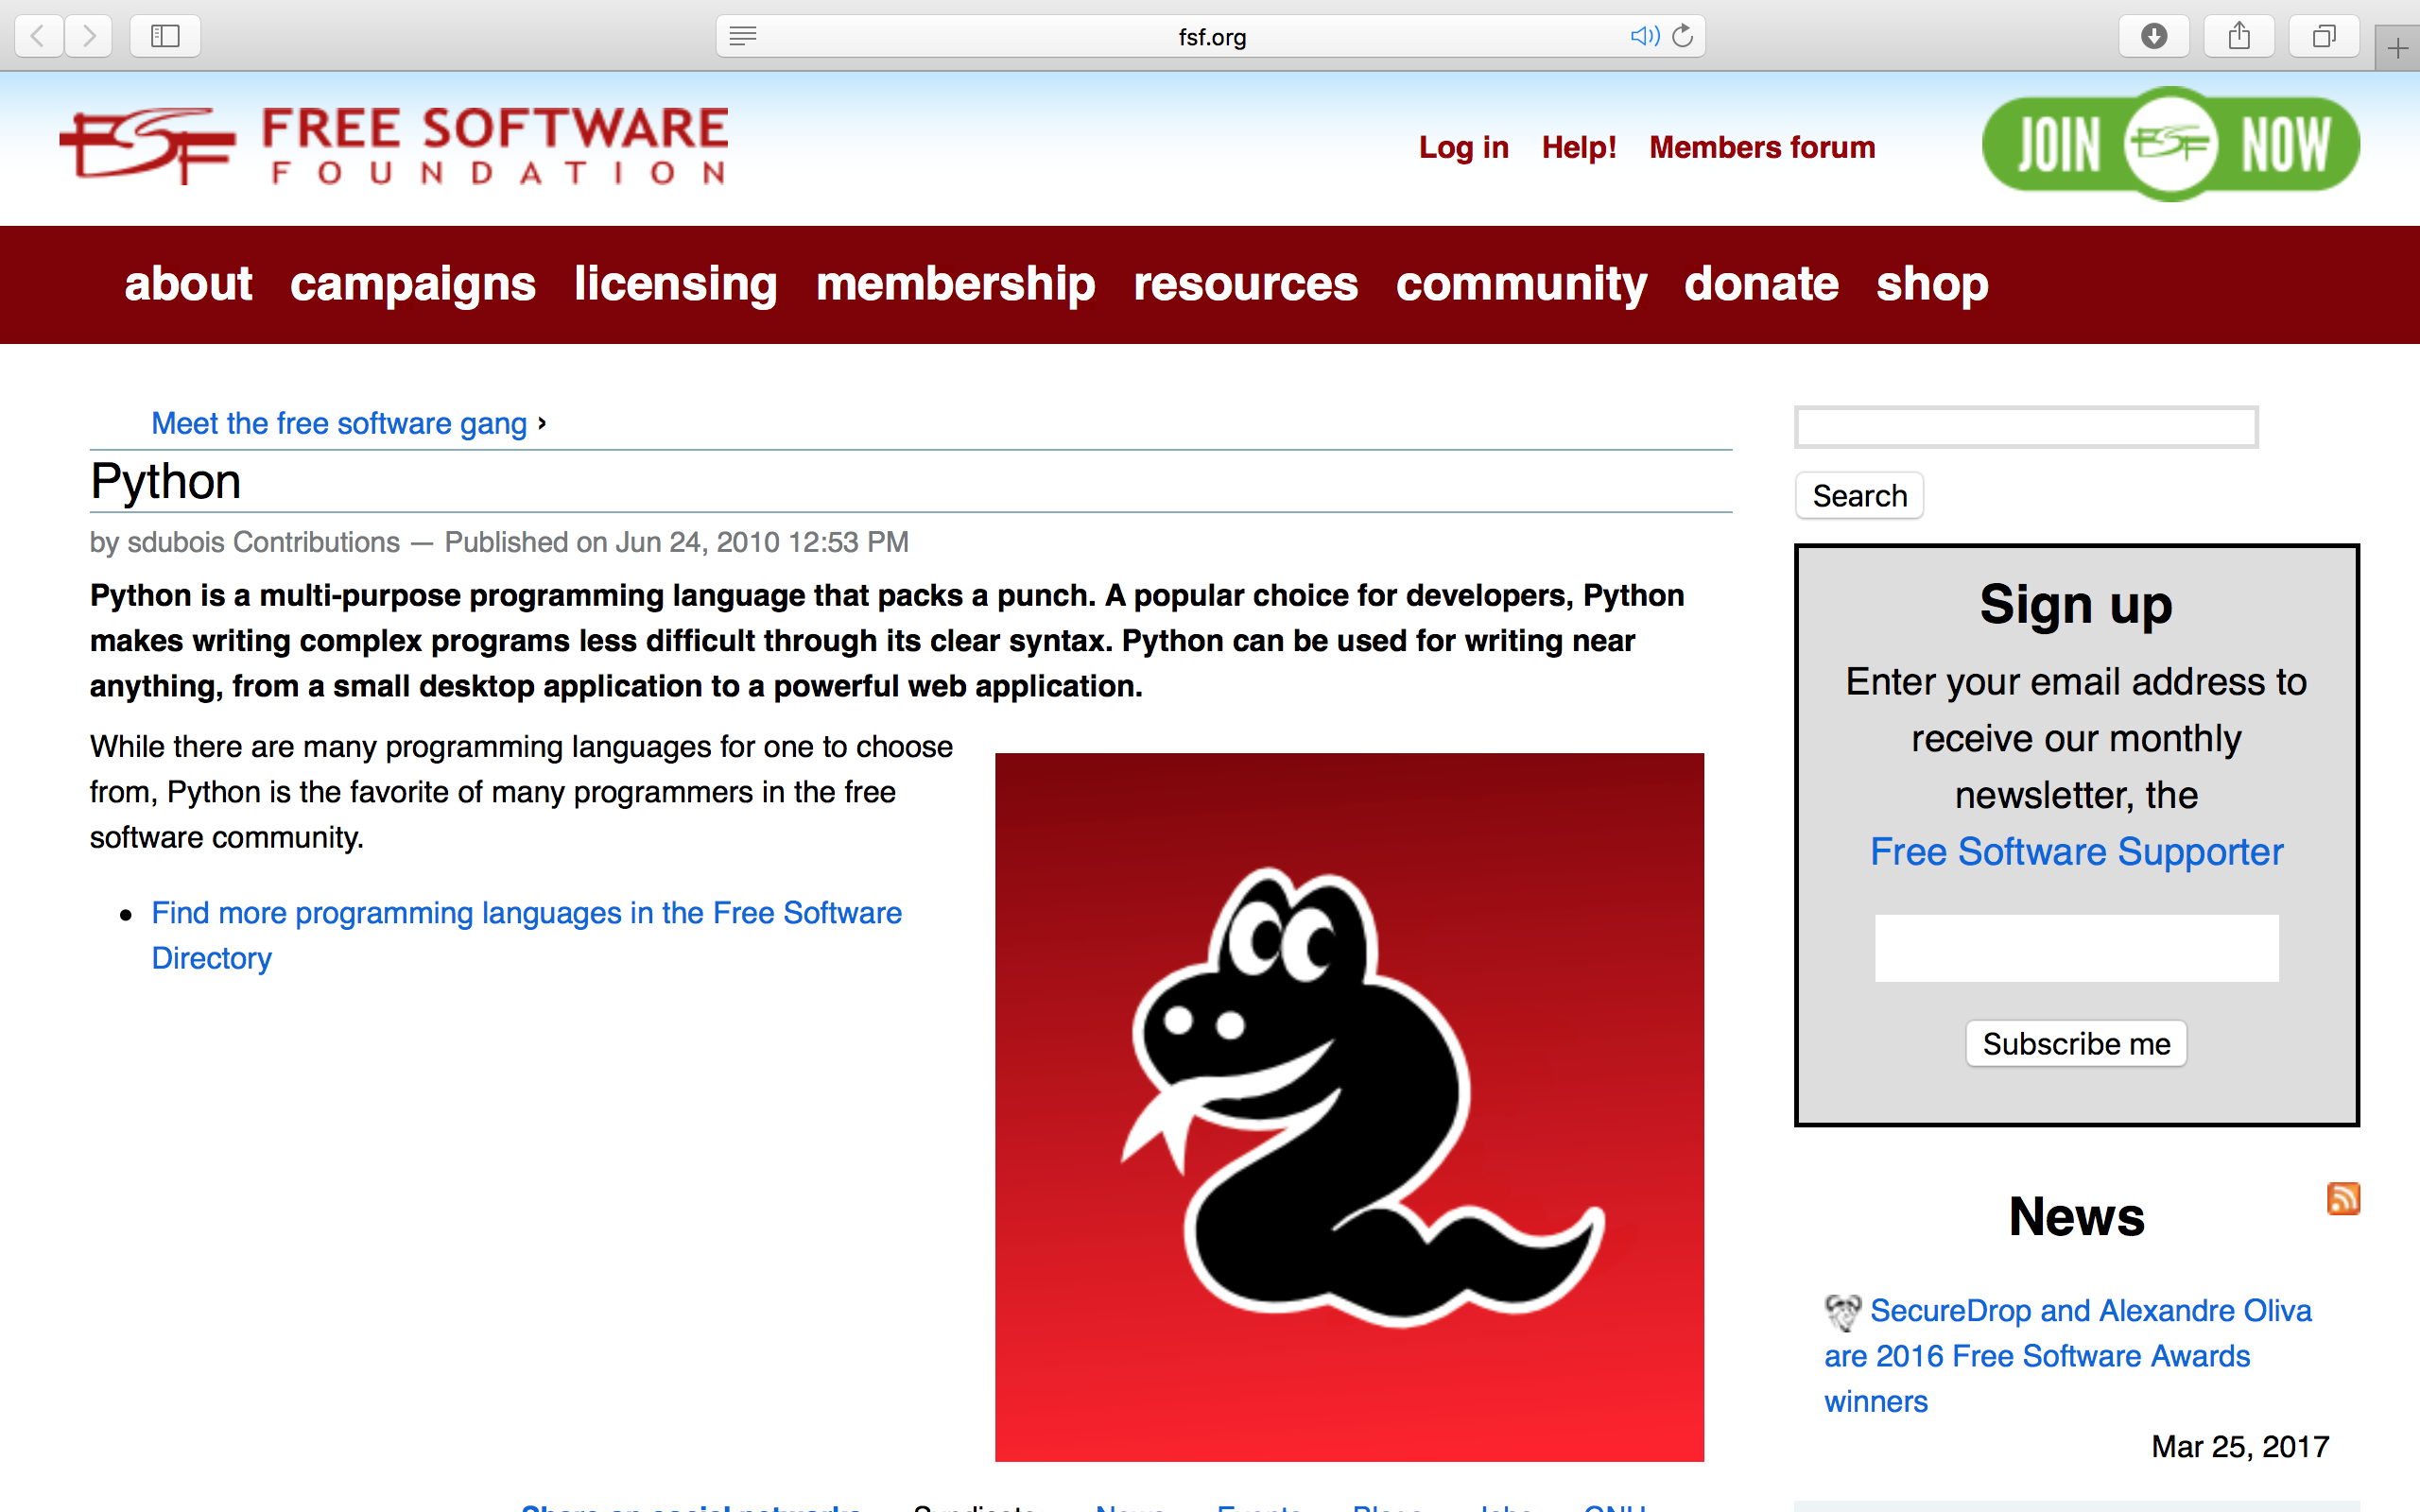
\includegraphics[scale=0.2]{imgs/fsf}
      \end{tcolorbox}
    \end{center}
  \end{frame}

  \begin{frame}{Recordando un poco...}
    Un \textbf{Software Libre} es aquel que respeta las cuatro libertades que
    la \textit{FSF} establece:
    \begin{itemize}
      \item La libertad de usar el programa con cualquier propósito.
      \item La libertad de estudiar cómo funciona el programa y modificarlo,
      adaptándolo a tus necesidades.
      \item La libertad de distribuir copias del programa, con lo cual puedes
      ayudar a tu prójimo.
      \item La libertad de mejorar el programa y hacer públicas esas mejoras a
      los demás, de modo que toda la comunidad se beneficie.
    \end{itemize}
    \textbf{Nota:} El Software Libre no es necesariamente gratuito.
  \end{frame}

  % Second section: Instalación
  \section{Instalación}
  \begin{frame}{Instalando Python}
    \begin{itemize}
      \item Ir al sitio oficial: \url{https://www.python.org/downloads/}
      \item Descargar la versión 3.x.x.
    \end{itemize}
    \begin{center}
      \begin{tcolorbox}[beamer,
                  width=1.065\textheight,
                  arc=0pt,
                  boxsep=0pt,
                  left=0pt,right=0pt,top=0pt,bottom=0pt,
                  ]
        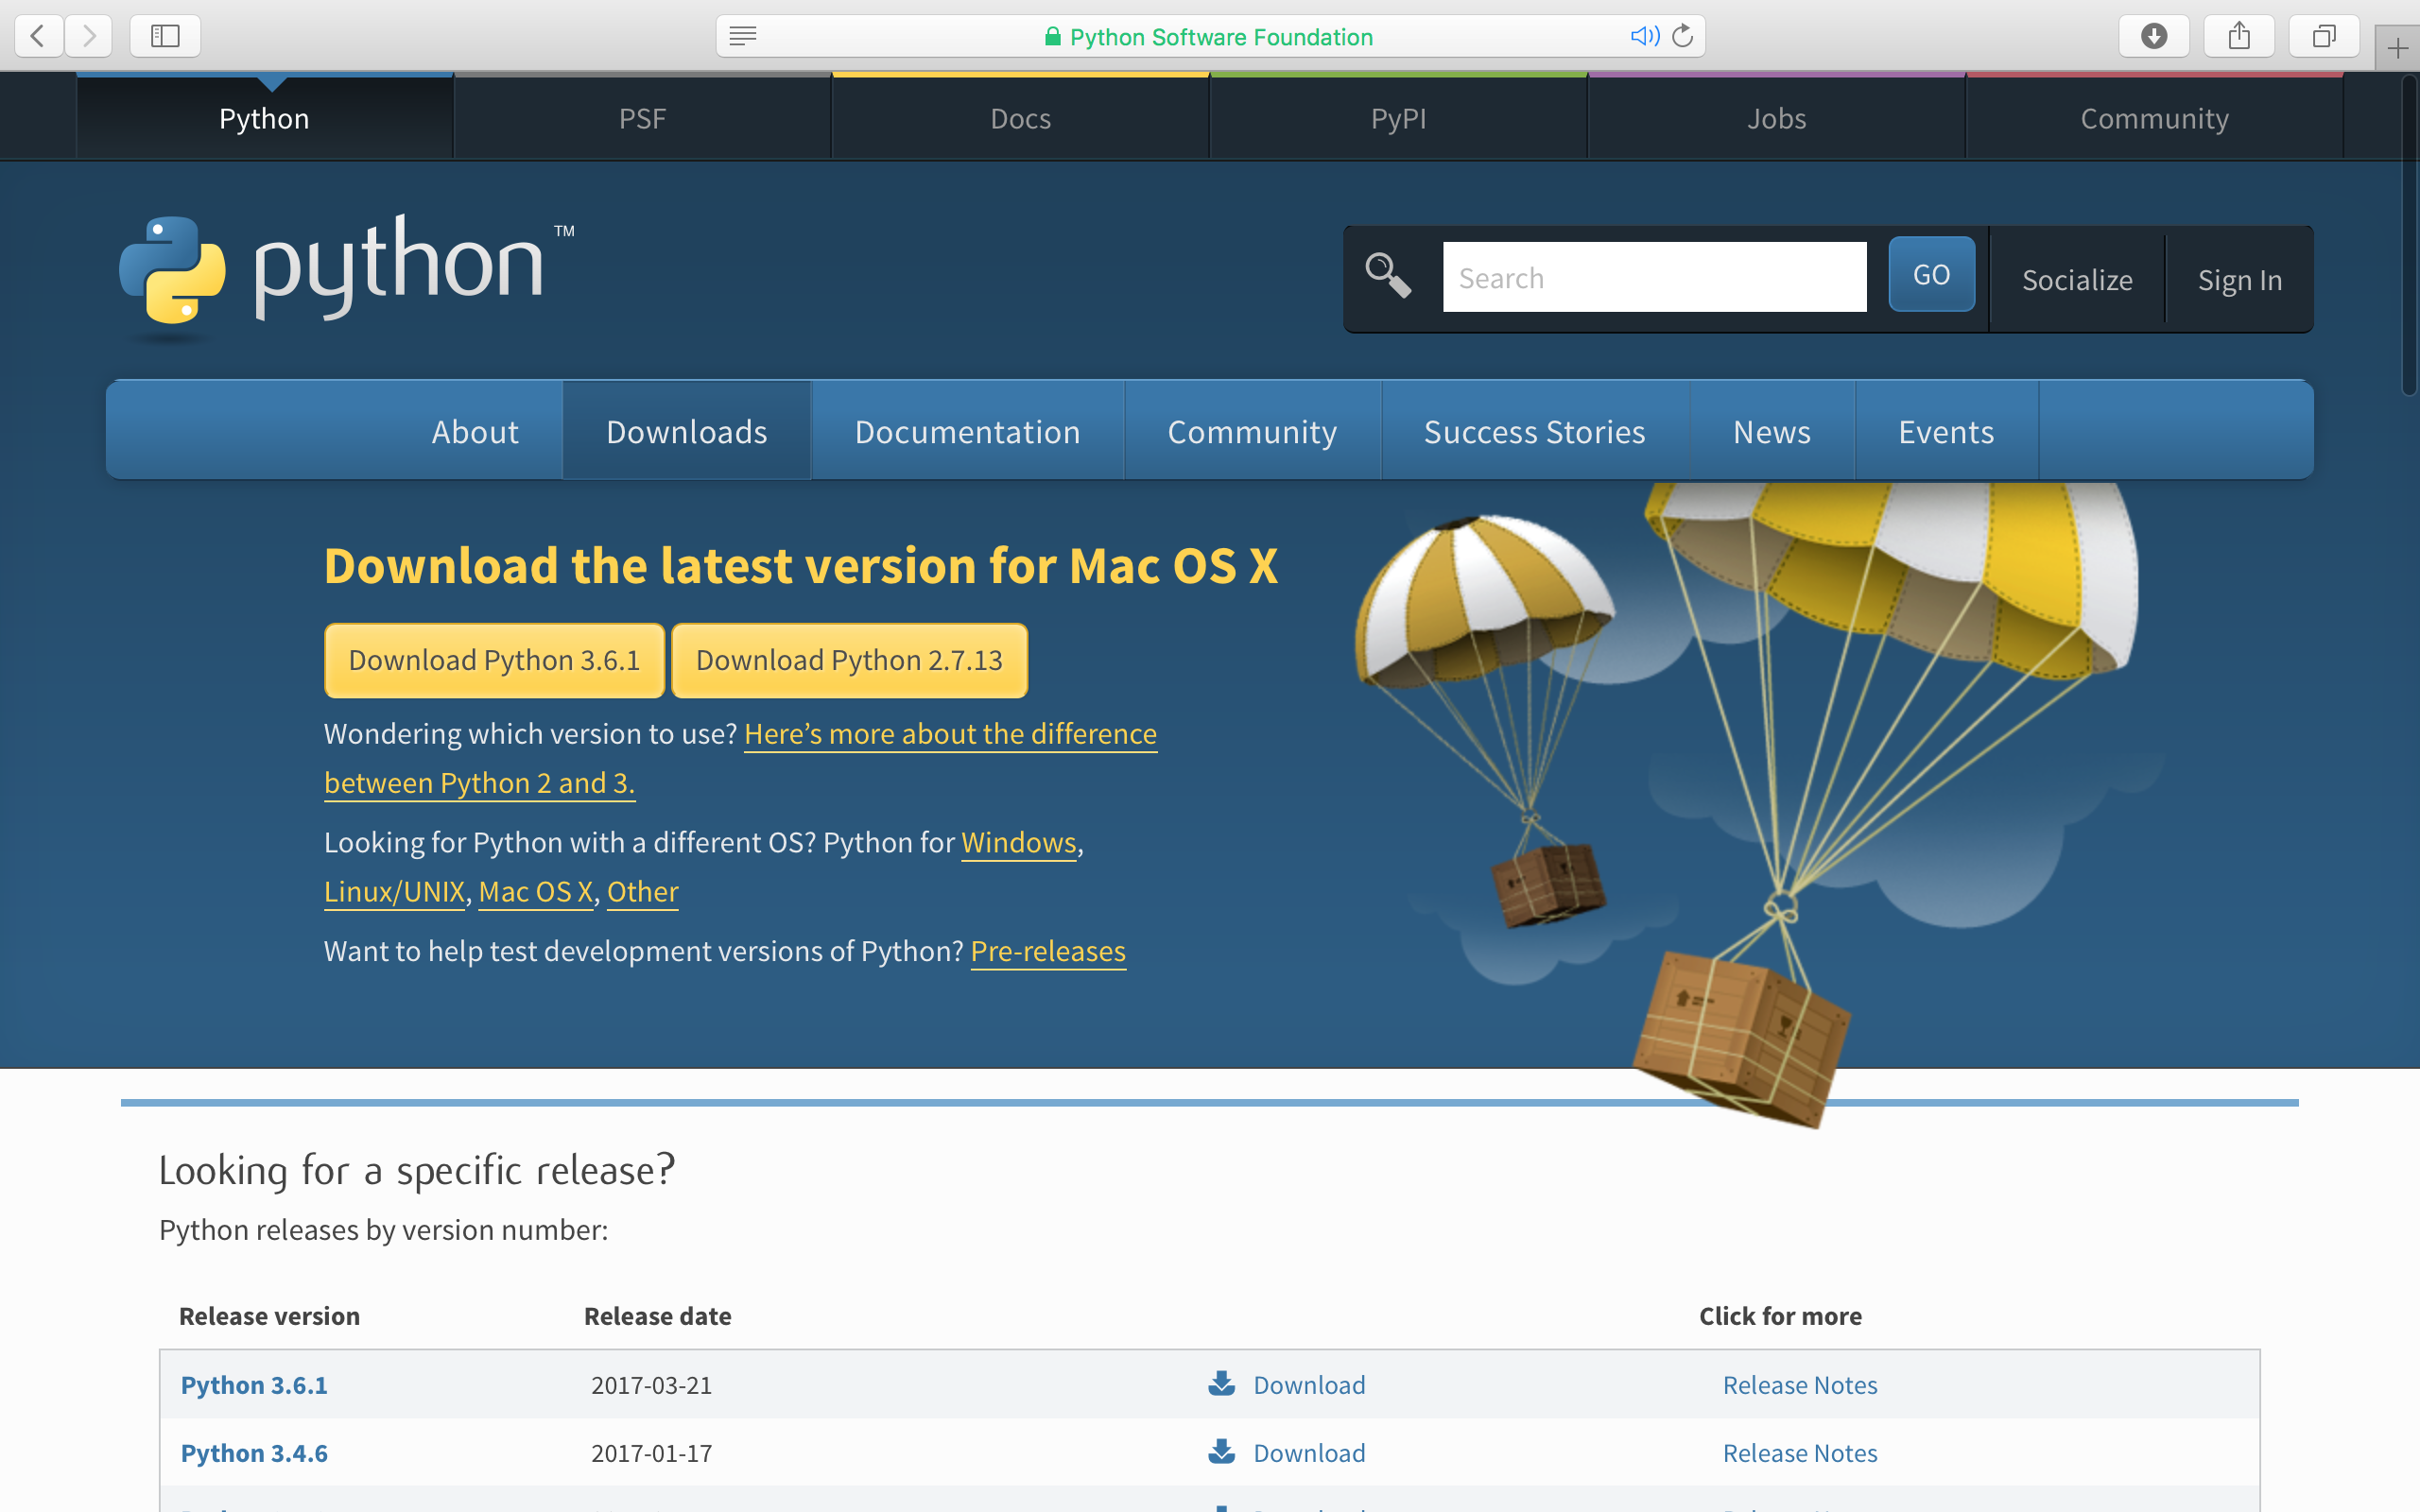
\includegraphics[scale=0.2]{imgs/download}
      \end{tcolorbox}
    \end{center}
  \end{frame}

  \begin{frame}{Instalando Python}
    \textbf{En Windows:}
    \begin{itemize}
      \item Preferentemente instalarlo en el disco local \texttt{C://}.
      \item Dar check a la opción de crear variable de entorno.
    \end{itemize}
    \textbf{En Linux/Unix:}
    \begin{itemize}
      \item No hace falta algo adicional, todo es hermoso.
      \item Es más, por default ya viene instalada la versión 2.7 de Python.
    \end{itemize}
  \end{frame}

  \begin{frame}{Instalando paquetes}
    Al instalar Python, se instala \texttt{pip} (\textit{Python Package Index}),
    que es un gestor de paquetes de Python. Usando \texttt{pip} instalaremos:
    \begin{itemize}
      \item \textbf{Numpy}, que incluye herramientas de métodos numéricos.
      \item \textbf{Matplotlib}, que incluye herramientas de visualización.
    \end{itemize}
    \textbf{Nota:} Python se instala con su librería estándar. Lo recomendable
    es instalar una distribución (como \textit{Anaconda}) para una mejor
    gestión de paquetes, además de instalarse por default los más usados.
  \end{frame}

  \begin{frame}{Paquetes de manipulación de imágenes}
    Existen diversos paquetes para manipular imágenes:
    \begin{itemize}
      \item \textbf{PIL} (\textit{Python Imaging Library})
      \item \textbf{OpenCV} (\textit{OpenSource Computer Vision})
      \item \textbf{scikit-image} (\textit{Scientific Kit - Image})
      \item Etc.
    \end{itemize}
    Cada uno trata de manera distinta las imágenes y se enfocan en cosas
    diferentes. Como es un taller de primeros pasos, no usaremos alguno de
    estos paquetes, sino que trabajaremos desde cero, sólo con \textbf{numpy}
    y \textbf{matplotlib}.
  \end{frame}

  \begin{frame}{Instalando \textbf{numpy} y \textbf{matplotlib}}
    Abriremos una consola y ejecutaremos los siguientes comandos.
    \metroset{block=fill}
    \begin{block}{Para instalar \textbf{numpy}:}
      \texttt{\$\hspace{0.3cm}sudo pip install numpy}
    \end{block}
    \vspace*{0.5cm}
    \begin{block}{Para instalar \textbf{matplotlib}:}
      \texttt{\$\hspace{0.3cm}sudo pip install matplotlib}
    \end{block}
    \textbf{Nota:} En Windows se omite el comando \texttt{sudo}.
  \end{frame}

  % Third section: Primeros pasos
  \section{Primeros pasos}
  \begin{frame}{Lo básico}
    
  \end{frame}

  % Fourth section: Manipulando imágenes
  \section{Manipulando imágenes}
  \begin{frame}{Objetivos}
    Queremos ser capaces de recrear las siguientes imágenes:
    \begin{center}
      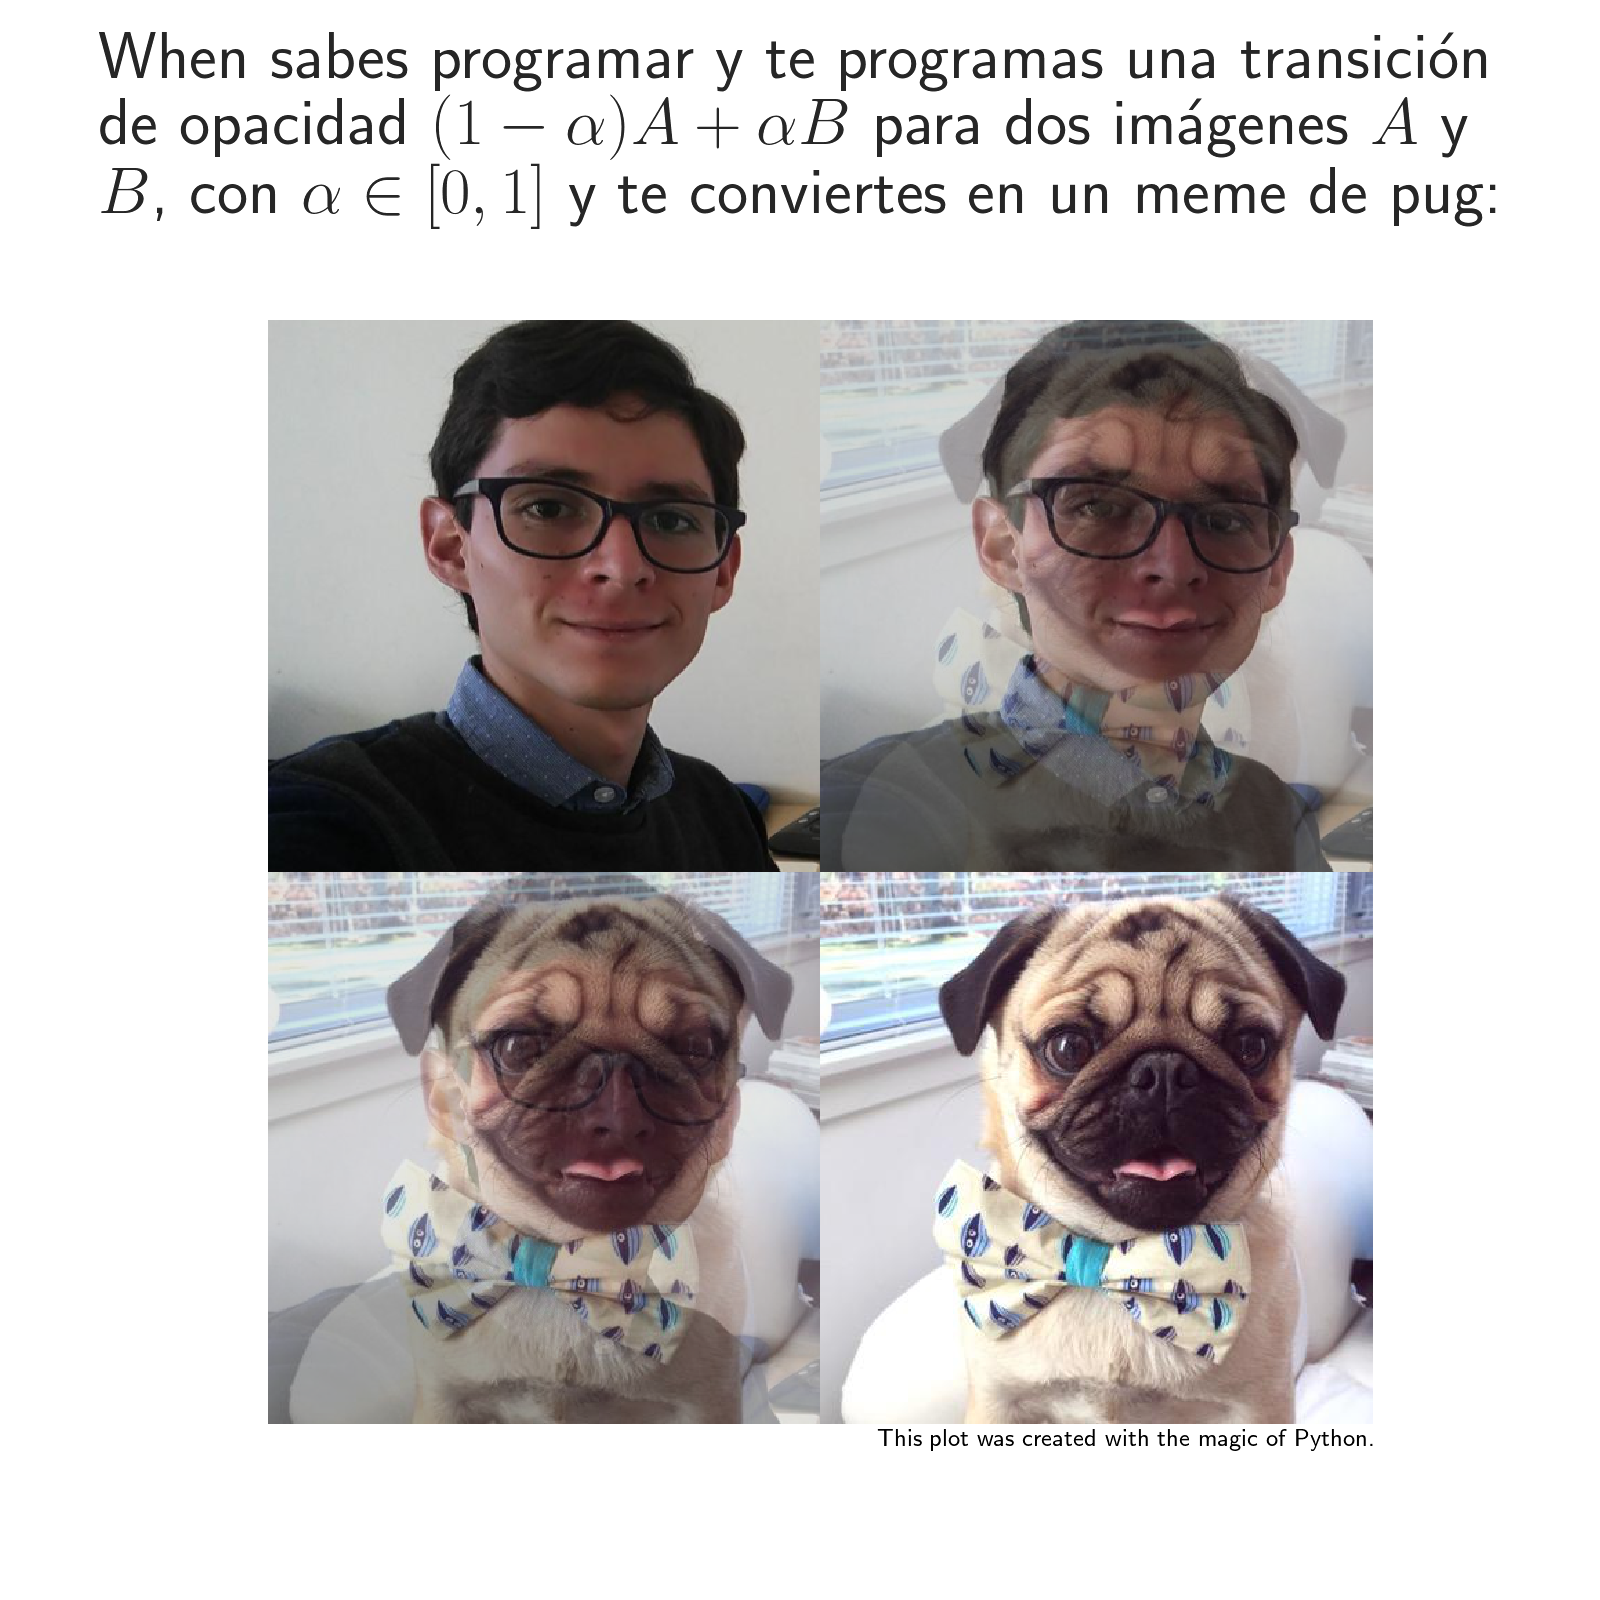
\includegraphics[width=0.48\textwidth]{imgs/meme}\hspace{0.1cm}
      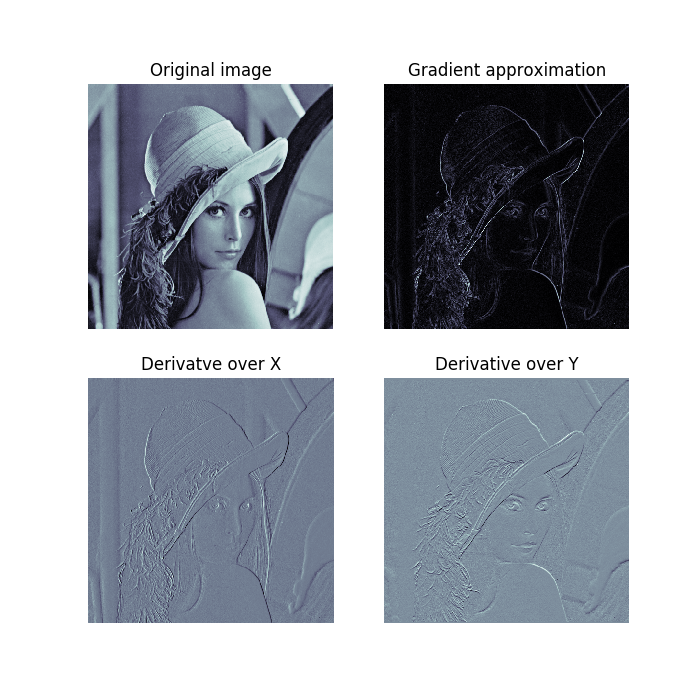
\includegraphics[width=0.48\textwidth]{imgs/derivatives}
    \end{center}
  \end{frame}

  % Fifth section: Creando imágenes
  \section{Creando imágenes}
  \begin{frame}{Objetivos}
    Queremos ser capaces de recrear la siguiente imagen:
    \begin{center}
      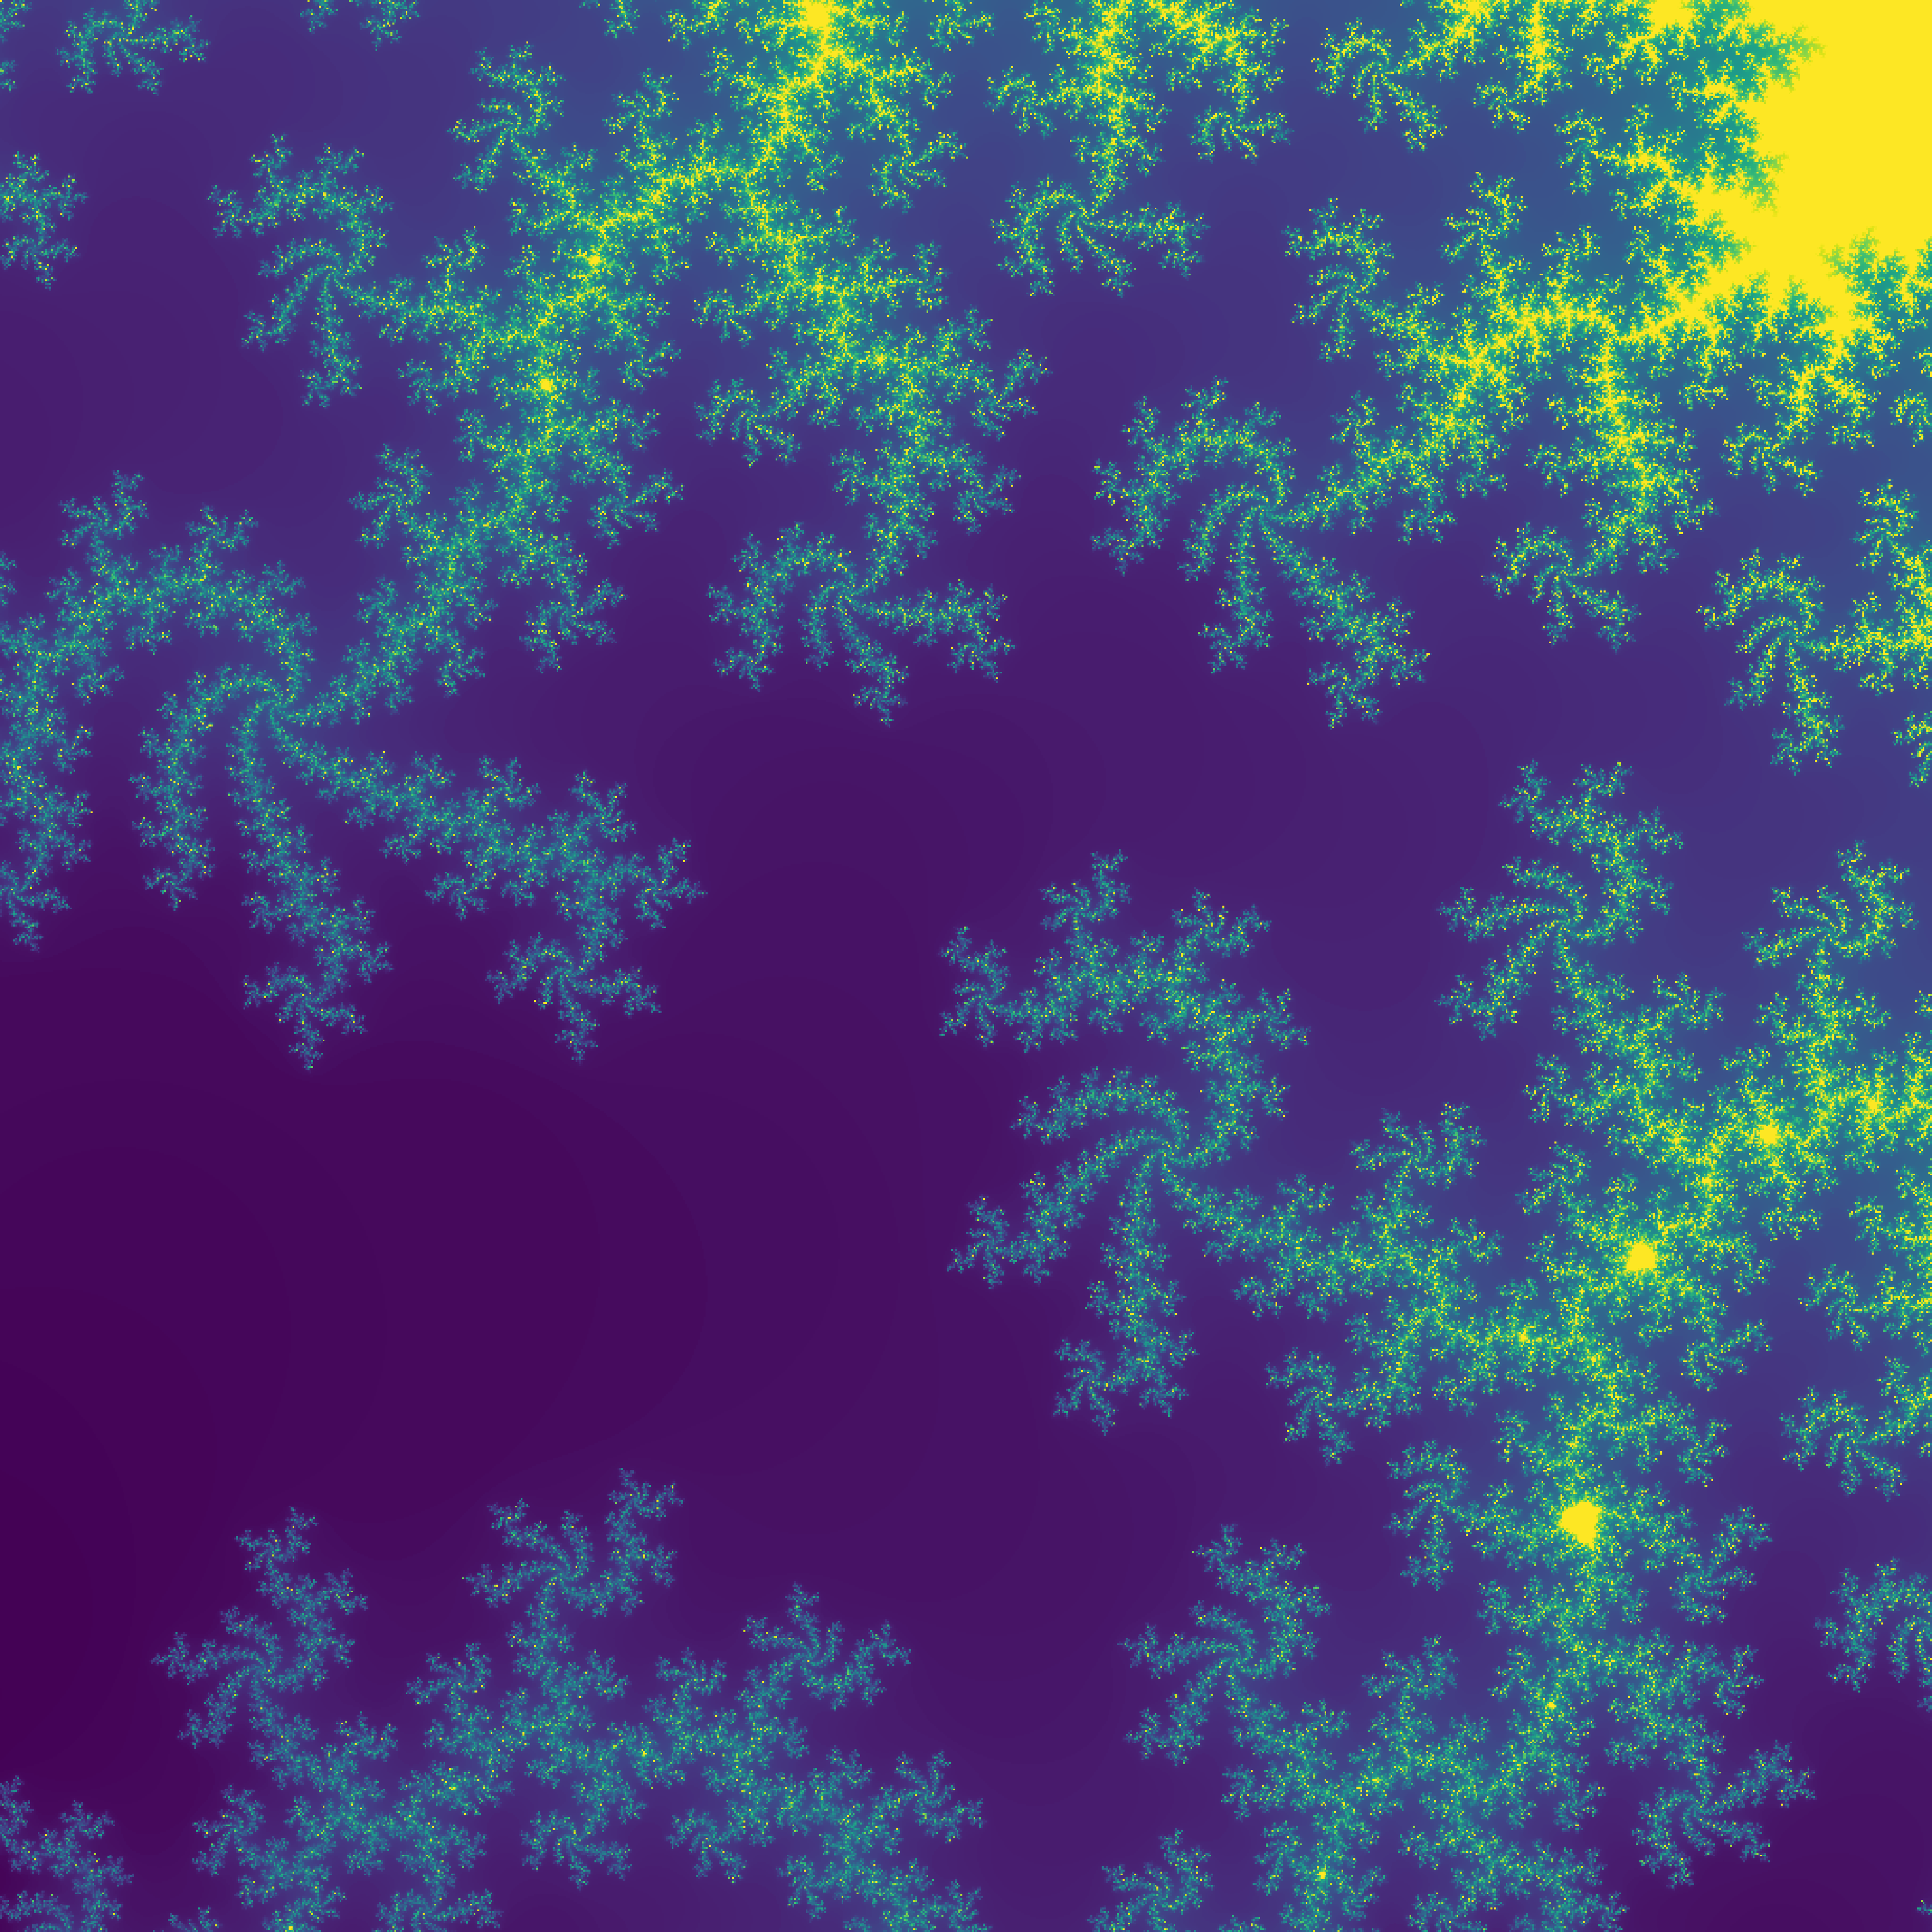
\includegraphics[width=0.6\textwidth]{imgs/mandel}\hspace{0.5cm}
    \end{center}
  \end{frame}

  % Questions
  \begin{frame}[standout]
    ¿Preguntas?
  \end{frame}

  % References
  \begin{frame}{Referencias}
    \begin{enumerate}[{[}1{]}]
      \item Python Software Foundation.\\
      \textbf{History of the software}.\\
      \textit{History and Licence},
      disponible en \texttt{https://docs.python.org/3/license.html}, 2017.

      \item Hipertextual.\\
      \textbf{¿Qué es Software Libre?}.\\
      \textit{Diferencias entre Software Libre y Open Source}, 2014.

      \item Hipertextual.\\
      \textbf{¿Qué es Open Source?}.\\
      \textit{Diferencias entre Software Libre y Open Source}, 2014.
    \end{enumerate}
  \end{frame}

  \begin{frame}{Referencias}
    \begin{enumerate}[{[}1{]}]
      \addtocounter{enumi}{3}

      \item The Hitchhiker's Guide to Python.\\
      \textbf{Python Imaging Library}.\\
      \textit{Image Manipulation}, 2016.

      \item The Hitchhiker's Guide to Python.\\
      \textbf{OpenSource Computer Vision}.\\
      \textit{Image Manipulation}, 2016.

      \item Third item
    \end{enumerate}
  \end{frame}
\end{document}
